\documentclass[conference]{IEEEtran}
\IEEEoverridecommandlockouts
\usepackage{cite}
\usepackage{amsmath,amssymb,amsfonts}
\usepackage{algorithmic}
\usepackage{graphicx}
\usepackage{textcomp}
\usepackage{xcolor}
\usepackage{booktabs}
\usepackage{multirow}
\usepackage{array}
\usepackage{comment}
\usepackage{url}
\usepackage{hyperref}

\graphicspath{{figures/}}

\def\BibTeX{{\rm B\kern-.05em{\sc i\kern-.025em b}\kern-.08em
    T\kern-.1667em\lower.7ex\hbox{E}\kern-.125emX}}

\begin{document}

\title{Diagnosing Test-Time Adaptation Failures in Multi-Instance Learning for Breast Cancer Histopathology}

\makeatletter
\newcommand{\linebreakand}{%
  \end{@IEEEauthorhalign}
  \hfill\mbox{}\par
  \mbox{}\hfill\begin{@IEEEauthorhalign}
}
\makeatother

%\author{
%\IEEEauthorblockN{Akib Hasan Pyil}
%\IEEEauthorblockA{
%\textit{Department of Computer Science} \\
%\textit{American International University-Bangladesh} \\
%Dhaka, Bangladesh \\
%23-50531-1@student.aiub.edu
%}
%\and
%\IEEEauthorblockN{Mohammad Rabib Uddin}
%\IEEEauthorblockA{
%\textit{Department of Electrical and Electronic Engineering} \\
%\textit{American International University-Bangladesh} \\
%Dhaka, Bangladesh \\
%rabib@aiub.edu
%}
%}
 
\maketitle

\begin{abstract}
Test-time adaptation (TTA) has reduced distribution-shift errors by up to 40\% on natural image benchmarks, motivating its application to computational pathology, where cross-site generalization remains a persistent deployment problem. We apply four TTA strategies -- entropy minimization (TENT), self-supervised auxiliary tasks (TTT), covariance alignment (CORAL), and a phased hybrid approach -- to Multi-Instance Learning (MIL) aggregators trained on the BACH breast histopathology dataset and evaluated on BreakHis without target labels. On BACH, UNI-based AB-MIL reaches 0.9700 accuracy and 0.9973 AUROC five times. Despite this strong source performance, none of the TTA methods improve cross-domain accuracy on BreakHis beyond the no-adaptation baseline. A supervised fine-tuning upper bound reaches 0.9250 accuracy with the same features, confirming that the features are suitable and the unsuccessful adaptation arises from the mechanism itself. We trace this observed behavior to a fundamental precondition violation: BACH trains a 4-class classifier while BreakHis requires a 2-class one, so the classification head is randomly re-initialized at transfer time. TTA updates only LayerNorm affine parameters and cannot recover a randomly initialized head. This result identifies a critical precondition, label-space compatibility between source and target that must hold for TTA to function in MIL settings, and provides concrete guidance for practitioners deploying MIL models across institutions.
\end{abstract}

\begin{IEEEkeywords}
test-time adaptation, multi-instance learning, breast cancer histopathology, domain generalization, weakly supervised learning
\end{IEEEkeywords}

\section{Introduction}

Computational pathology models do not travel well. A Multi-Instance Learning (MIL) classifier trained on slides from one institution commonly loses five to twenty percentage points when evaluated on slides from another, due to scanner differences, staining variation, and demographic shifts \cite{chen2022scaling, lu2021data}. This is not a theoretical concern; it is a routine obstacle to clinical deployment, and it happens even when the underlying task is identical at both sites.

Test-time adaptation (TTA) updates a small subset of model parameters at inference time using only the unlabeled test sample, requiring no target-domain labels, no retraining, and no access to source data beyond what was already baked into the trained model. On natural image corruption benchmarks, TENT reduces classification error by up to 40\%, and more recent methods push further \cite{niu2023towards, liu2021ttt, wang2022cotta, niu2022eata, yuan2023rotta}. The promise is label-free adaptation at test time with no retraining cost.

Applying TTA to MIL introduces complications that the TTA literature has not addressed. In MIL, the inference unit is a bag of patches, typically 32 to thousands per slide. Bag-level entropy is noisier than single-image entropy, and the attention aggregator introduces a pooling step that TTA was not designed around. None of these properties is obviously favorable for entropy minimization or covariance alignment.

The pathology community has not systematically asked whether TTA works for MIL, under what conditions, and why it might fail. This paper provides that study. We implement TENT, TTT, CORAL, and Hybrid TTA for three MIL aggregators (AB-MIL, TransMIL, CLAM) trained on BACH with ResNet-50 and UNI features, and evaluate cross-domain transfer to BreakHis \cite{spanhol2016dataset}. The result is a null: TTA produces no meaningful improvement in this setting.

The more important contribution is the diagnosis. We trace the limitation to a precondition that TTA literature takes for granted, label-space compatibility between source and target. BACH is 4-class; BreakHis is binary. The classification head is replaced and randomly re-initialized at transfer time, and TTA, updating only LayerNorm affine parameters, has no path to recover a random output layer. A supervised fine-tuning upper bound with 30\% labeled target samples reaches 0.9250 accuracy, confirming the features are rich enough and the limitation is structural.

The contributions of this paper are: (1) the first systematic TTA study for MIL, (2) a rigorous null result with root-cause diagnosis (0.9250 vs. 0.19 for label-free TTA), (3) a three-precondition checklist for TTA in MIL, and (4) strong source-domain baselines (UNI-based AB-MIL achieves 0.9700 accuracy and 0.9973 AUROC on BACH).



\section{Related Work}
\label{sec:related}

\subsection{Multiple Instance Learning for Pathology}

Ilse et al. \cite{ilse2018attention} introduced the gated attention MIL aggregator (AB-MIL) that most current methods descend from, demonstrating that attention-based pooling can identify discriminative patches without patch-level labels. CLAM \cite{lu2021data} extended this with instance-level clustering supervision, substantially improving performance on five TCGA tasks. TransMIL \cite{shao2021transmil} replaced attention pooling with a Transformer encoder, capturing spatial dependencies that the original attention mechanism misses. Chen et al. \cite{chen2022scaling} scaled these ideas to multi-task, multi-cohort settings.

Pathology foundation models have changed what is achievable on small labeled datasets. UNI \cite{chen2024uni}, Virchow2, GigaPath, and CONCH provide frozen patch encoders that transfer substantially better than ImageNet-pretrained ResNets. Chen et al. \cite{chen2024uni} showed UNI achieves state-of-the-art on 34 of 34 benchmarks; our source-domain results corroborate this on BACH. The cross-site generalization problem, however, remains unsolved at the aggregator level regardless of encoder quality.

\subsection{Test-Time Adaptation}

TENT \cite{wang2021tent} is the most widely cited TTA method: it minimizes prediction entropy using only normalization affine parameter updates. It assumes source and target label spaces are the same. TTT \cite{sun2020test} trains a self-supervised auxiliary head jointly with the main task so the auxiliary gradient can update the encoder at test time. CORAL \cite{sun2016coral} aligns second-order feature statistics between domains; in TTA form, this is computed from the test bag alone against stored source statistics.

More recent methods address failure modes: CoTTA \cite{wang2022cotta} introduces weight averaging for continual adaptation; EATA \cite{niu2022eata} employs entropy-based sample selection; RoTTA \cite{yuan2023rotta} uses prototype-based pseudo-labeling; MEMO \cite{zhang2022tip} improves robustness via test-time augmentation; AdaContrast \cite{chen2022adacontrast} leverages contrastive learning for online adaptation. SAR \cite{niu2023towards} and TTT++ \cite{liu2021ttt} improve stability under heavy or time-varying shifts. All these methods share the assumption that the output mapping at the source is meaningful for the target task---an assumption that fails when label spaces differ between source and target domains.

\subsection{Cross-Domain Generalization in Pathology}

Stain normalization \cite{macenko2009method} is the most common preprocessing approach for cross-site transfer, but it addresses only staining shift. The most directly relevant prior work is STAMP \cite{chen2023stamp}, which applies TTA to a slide-level encoder, but it does not operate within a MIL framework, evaluates only a single TTA strategy, and does not examine label-space conditions. To the best of our knowledge, no prior study has applied or evaluated TTA for MIL-based histopathology classification.

\begin{table*}[!htpb]
\centering
\caption{Summary of related studies on MIL, TTA, and cross-domain generalization}
\label{tab:related_work}
\resizebox{\textwidth}{!}{%
\begin{tabular}{c c p{3.6cm} p{2.8cm} p{2.6cm} p{4.0cm}}
\toprule
\textbf{Ref.} & \textbf{Year} & \textbf{Method} & \textbf{Dataset} & \textbf{Results} & \textbf{Limitations} \\
\midrule
\cite{ilse2018attention} & 2018 & Gated attention MIL & MNIST-Bags, Colon Cancer & AUROC 0.87 & No cross-site eval; no TTA \\
\cite{lu2021data} & 2021 & CLAM & TCGA (5 tasks) & AUC 0.868--0.985 & Trained/tested within TCGA \\
\cite{shao2021transmil} & 2021 & TransMIL & CAMELYON16, TCGA & AUC up to 0.931 & No domain generalization \\
\cite{chen2024uni} & 2024 & UNI + MIL & 34 pathology benchmarks & SOTA on all tested & No TTA; cross-dataset TTA not studied \\
\cite{wang2021tent} & 2021 & TENT & CIFAR-10-C, ImageNet-C & Error reduced 18--40\% & Natural images; same label space assumed \\
\cite{sun2020test} & 2020 & TTT & CIFAR-10, ImageNet & Error reduced 10--24\% & Joint training; single-image inference \\
\cite{wang2022cotta} & 2022 & CoTTA & CIFAR-10-C, ImageNet-C & Improved continual adaptation & Natural images only \\
\cite{chen2023stamp} & 2023 & TTA for slide-level encoder & TCGA & Improved calibration & Not MIL-based; single TTA strategy \\
Ours & 2025 & TENT/TTT/CORAL/Hybrid TTA for MIL & BACH, BreakHis & Null result; root cause identified & Label-space mismatch in current setup \\
\bottomrule
\end{tabular}}
\end{table*}

\section{Materials and Methods}
\label{sec:method}

\subsection{Datasets}

\textbf{BACH} \cite{aresta2019bach} is the ICIAR 2018 breast cancer histology challenge dataset. It contains 400 microscopy images (2048$\times$1536 pixels) across four balanced classes: Normal, Benign, InSitu, and Invasive carcinoma (100 images per class). It is used as the source domain throughout.

\textbf{BreakHis} \cite{spanhol2016dataset} contains biopsy images from 82 patients across four magnification factors (40X, 100X, 200X, 400X), with binary benign/malignant labels. The full dataset spans 31,636 images across all magnifications. Cross-domain evaluation uses the 200X subset ($n \approx 7{,}909$); the full multi-magnification set is used for ablation subsampling.

The critical difference is label space: BACH has four classes; BreakHis has two. This mismatch is the binding constraint analyzed in Section~\ref{sec:discussion}.

\begin{table}[!hbt]
\caption{Dataset Characteristics}
\label{tab:datasets}
\centering
\begin{tabular}{p{0.16\linewidth} p{0.26\linewidth} p{0.44\linewidth}}
\toprule
\textbf{Dataset} & \textbf{Role} & \textbf{Key characteristics} \\
\midrule
BACH \cite{aresta2019bach} & Source (train/val) & 400 images; 4 balanced classes; 2048$\times$1536 px; challenge microscopy \\
BreakHis \cite{spanhol2016dataset} & Target (test only) & 7,909 images (200X); 2 classes; biopsy; 82 patients \\
\bottomrule
\end{tabular}
\end{table}

\begin{figure}[!hbt]
  \centering
  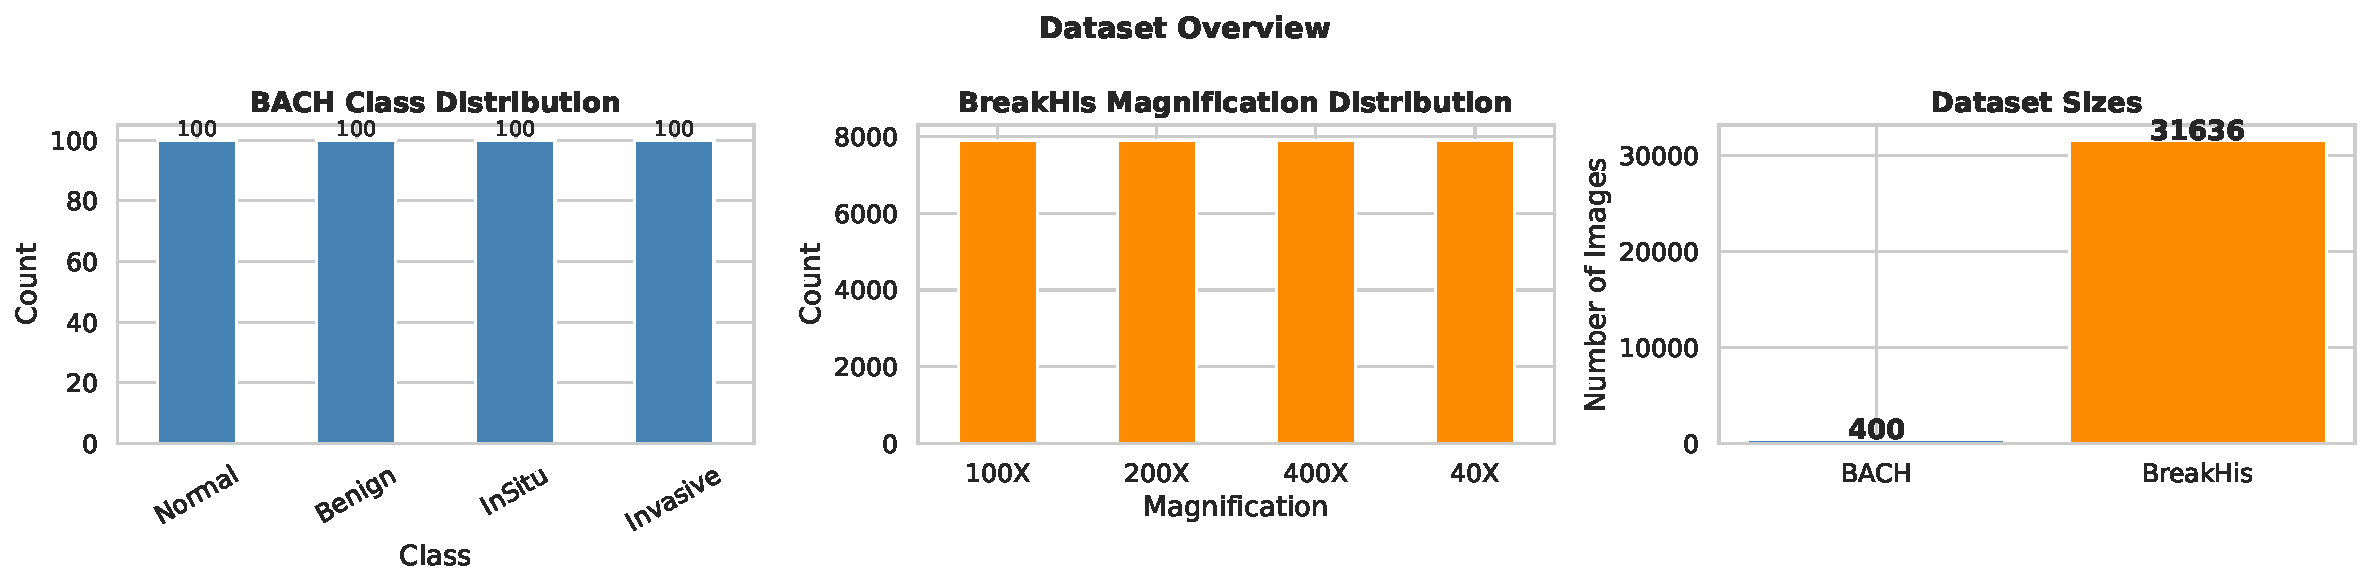
\includegraphics[width=\linewidth]{dataset_eda.pdf}
  \caption{Dataset overview. Left: BACH class distribution. Center: BreakHis image count across the four magnification factors. Right: total dataset sizes}
  \label{fig:dataset_eda}
\end{figure}

\subsection{Patch Extraction and Feature Encoding}

Each image is divided into 256$\times$256 patches with a stride of 128 pixels. Patches with mean pixel intensity above 230 are discarded as near-white background, consistent with standard H\&E tissue selection practice \cite{lu2021data, macenko2009method}.

Up to 32 patches per image are retained, following common practice in MIL for histopathology \cite{ilse2018attention, lu2021data}, balancing spatial coverage against GPU memory constraints.

Two feature extractors are compared:

\begin{itemize}
    \item \textbf{ResNet-50}: ImageNet pretrained, 2048-dim features, 23.5M parameters. General-purpose baseline.
    \item \textbf{UNI} \cite{chen2024uni}: ViT-L/16 pretrained on $>$100,000 H\&E pathology tiles, 1024-dim features, 303.4M parameters. Loaded from \texttt{hf-hub:MahmoodLab/uni}; frozen throughout all experiments.
\end{itemize}

Features are extracted offline and cached to HDF5 files (ResNet-50: 102.5 GB; UNI: 51.3 GB combined), so every method sees identical patch representations.

\subsection{MIL Aggregators}

\textbf{AB-MIL} \cite{ilse2018attention}: Attention-Based Multiple Instance Learning uses gated attention pooling with a two-layer MLP. Attention weights are produced via element-wise products of tanh and sigmoid branches over the patch features, followed by a softmax normalization. The resulting weighted sum forms the bag representation fed to the classifier.

\textbf{TransMIL} \cite{shao2021transmil}: Transformer-based MIL uses a two-layer Transformer encoder with a learnable CLS token. Patch features are projected to 512 dimensions, and the CLS token embedding after encoding is fed to the classifier.

\textbf{CLAM-SB} \cite{lu2021data}: Clustering-constrained Attention Multiple Instance Learning (single-branch) uses $k=8$ instance supervision. During training, the top-$k$ and bottom-$k$ attention-weighted patches receive pseudo-labels, adding an instance-level clustering loss to the bag-level cross-entropy objective.

All three use LayerNorm throughout. BatchNorm1d is avoided because batch statistics cannot be estimated from a single bag, making it unstable for test-time normalization updates.

\subsection{Source-Domain Training}

All aggregators are trained with 5-fold stratified cross-validation on BACH using AdamW \cite{loshchilov2019decoupled} with $\text{lr}=10^{-4}$, weight decay $10^{-4}$, cosine annealing, and label smoothing of 0.1. Each fold trains for 50 epochs, batch size 8 bags. The best checkpoint per fold (by validation accuracy) is saved; the fold with the highest validation accuracy provides the model for all cross-domain experiments.

Hyperparameters follow standard MIL practice \cite{lu2021data, shao2021transmil}. The TTA learning rate of $10^{-5}$ is one order of magnitude lower than the training rate to prevent destabilizing the source model \cite{wang2021tent}. Full configuration is in Table~\ref{tab:training}.

\begin{table}[!hbt]
\caption{Training and TTA Configuration}
\label{tab:training}
\centering
\begin{tabular}{p{0.36\linewidth} p{0.54\linewidth}}
\toprule
\textbf{Item} & \textbf{Setting} \\
\midrule
Framework & PyTorch 2.x, timm $\geq$0.9.12 \\
Patch size / stride & 256 px / 128 px \\
Max patches per bag & 32 \\
Loss / Optimizer & Cross-entropy (ls 0.1) / AdamW \\
LR (train / TTA) & $10^{-4}$ / $10^{-5}$ \\
Batch size / Epochs & 8 bags / 50 \\
TTA updated parameters & LayerNorm $\gamma$, $\beta$ only \\
TTA steps per bag & $\leq$10; reset between bags \\
CV folds & 5-fold stratified \\
Hardware & NVIDIA Tesla T4, 15.6 GB \\
\bottomrule
\end{tabular}
\end{table}

\subsection{Test-Time Adaptation Methods}

All four TTA methods update only the LayerNorm affine parameters ($\gamma$, $\beta$), following the TENT framework \cite{wang2021tent}: they are low-dimensional, control intermediate representation scale where normalization statistics diverge under shift, and limit catastrophic forgetting. Encoders and attention weights are frozen. Each bag is adapted independently, with parameters reset after each bag to prevent cross-bag contamination.

\textbf{TENT} \cite{wang2021tent}: Test-Time Entropy Minimization minimizes bag-level prediction entropy $H(p) = -\sum_c p_c \log p_c$ for $n$ gradient steps before the final prediction is read off.

\textbf{TTT} \cite{sun2020test}: Test-Time Training adds a self-supervised auxiliary loss to TENT. Operating on pre-extracted features (not raw pixels), rotation is approximated by circular channel permutation: the feature vector is rolled by $d/4$ positions for each of four pseudo-angle indices. A lightweight linear head predicts which permutation was applied:
\begin{equation}
\mathcal{L}_{\text{TTT}} = H(p) + \lambda \mathcal{L}_{\text{rot}}, \quad \lambda = 0.5
\end{equation}

\textbf{CORAL} \cite{sun2016coral}: Correlation Alignment minimizes the Frobenius distance between source and target feature covariance matrices. Source covariance is pre-computed once from a fixed, seeded pool of 4,096 source patches (not resampled per test bag):
\begin{equation}
\mathcal{L}_{\text{CORAL}} = \frac{1}{4d^2} \| C_S - C_T \|_F^2
\end{equation}
Combined loss: $\mathcal{L} = H(p) + \lambda \mathcal{L}_{\text{CORAL}}$.

\textbf{Hybrid}: steps 1--3 apply TENT only to stabilize normalization statistics; steps 4--10 add the CORAL alignment loss and TTT rotation loss simultaneously. This phased approach prevents covariance alignment from amplifying noisy early entropy gradients.

\begin{figure*}[!t]
  \centering
  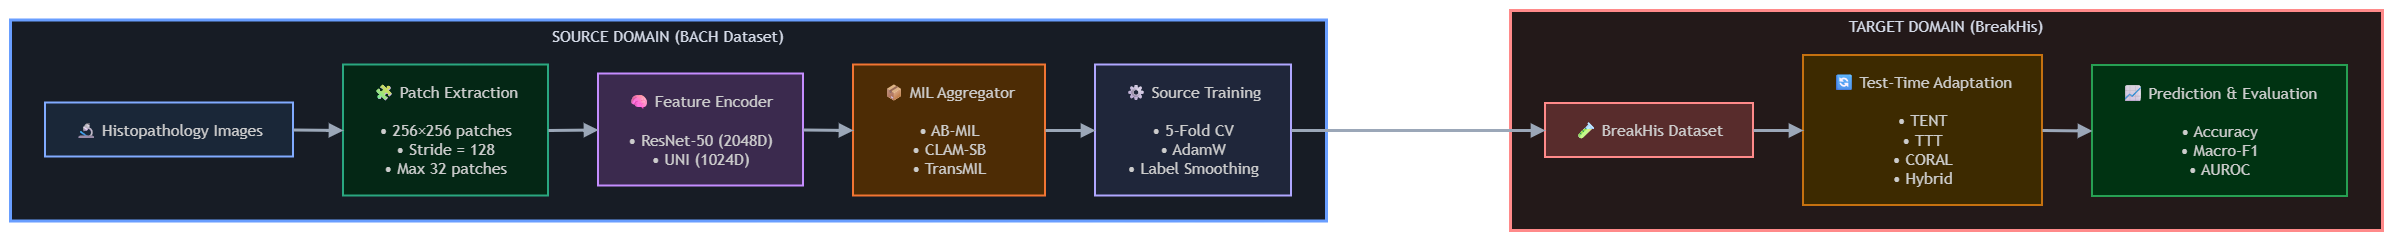
\includegraphics[width=\linewidth]{fig_method.png}
  \caption{Overall methodology of the proposed TTA-MIL framework.}
  \label{fig:method}
\end{figure*}

\subsection{Evaluation Protocol}

Two scenarios are evaluated:
\begin{itemize}
    \item \textbf{S1}: BACH$\rightarrow$BACH held-out (best fold validation set, $n=80$)
    \item \textbf{S2}: BACH$\rightarrow$BreakHis 200X ($n \approx 7{,}909$)
\end{itemize}

For BreakHis, the source model's 4-class head is replaced with a randomly initialized 2-class linear layer. This matches real deployment conditions where the target classification schema differs from the source. Metrics are accuracy, macro-F1, and macro-AUROC. Paired McNemar's tests compare each TTA method against no-adaptation on the same samples.

The dataset split is image-wise (BACH provides no patient identifiers). To mitigate leakage, splitting uses a fixed seed (42), stratified sampling, and no overlapping patches between train and validation sets.

\subsection{Ablation Study}

Six ablation conditions on a stratified 600-sample BreakHis subset:

\begin{itemize}
    \item \textbf{A1}: No TTA (0 adaptation steps)
    \item \textbf{A2}: TENT, 1 step
    \item \textbf{A3}: TENT, 10 steps
    \item \textbf{A4}: TTT only, 5 steps
    \item \textbf{A5}: CORAL only, 5 steps
    \item \textbf{A6}: Supervised fine-tuning on 30\% of the 600-sample ablation subset (180 images), 5 epochs
\end{itemize}

A6 uses labels and is not a fair comparison with TTA; it is included solely to establish an upper bound on what the extracted features can achieve with a properly fitted head. The 30\% fraction applies to the same 600-sample stratified subset used in A1--A5, not the full BreakHis dataset.

\section{Results}
\label{sec:results}

\subsection{Source-Domain Performance on BACH}

Table~\ref{tab:source_domain} reports 5-fold CV results. With ResNet-50, TransMIL reaches 0.8900 accuracy; CLAM-SB is weakest at 0.8175. With UNI, all three aggregators exceed 0.9625 accuracy and all AUROC values exceed 0.995. The backbone gap is 0.08--0.15 accuracy points; the aggregator gap within each backbone is small (UNI: $<$0.01, ResNet-50: 0.07). On small pathology datasets, encoder quality matters more than aggregator design.

\begin{table}[!hbt]
\caption{5-Fold CV Source-Domain Performance on BACH}
\label{tab:source_domain}
\centering
\begin{tabular}{llccc}
\toprule
\textbf{Backbone} & \textbf{Aggregator} & \textbf{Acc.} & \textbf{Macro-F1} & \textbf{AUROC} \\
\midrule
\multirow{3}{*}{ResNet-50}
 & TransMIL   & 0.8900 & 0.8895 & 0.9625 \\
 & AB-MIL     & 0.8475 & 0.8443 & 0.9440 \\
 & CLAM-SB    & 0.8175 & 0.8139 & 0.9434 \\
\midrule
\multirow{3}{*}{UNI}
 & AB-MIL     & \textbf{0.9700} & \textbf{0.9700} & \textbf{0.9973} \\
 & CLAM-SB    & 0.9675 & 0.9675 & 0.9953 \\
 & TransMIL   & 0.9625 & 0.9623 & 0.9958 \\
\bottomrule
\end{tabular}
\end{table}

%\begin{figure}[!hbt]
%  \centering
 % 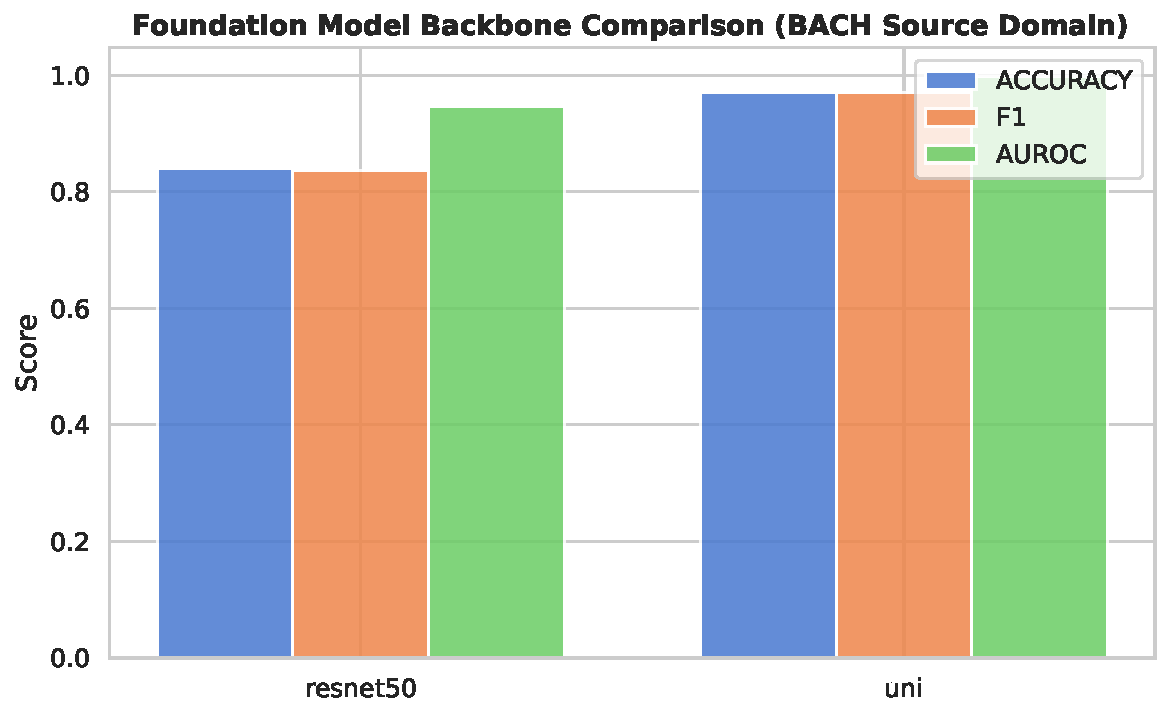
\includegraphics[width=\linewidth]{backbone_comparison.pdf}
 % \caption{Foundation model backbone comparison on the BACH source domain (5-fold CV). UNI outperforms ResNet-50 by 0.08--0.15 accuracy points across all three aggregators.}
 % \label{fig:backbone_comparison}
%\end{figure}

\begin{figure}[!hbt]
  \centering
  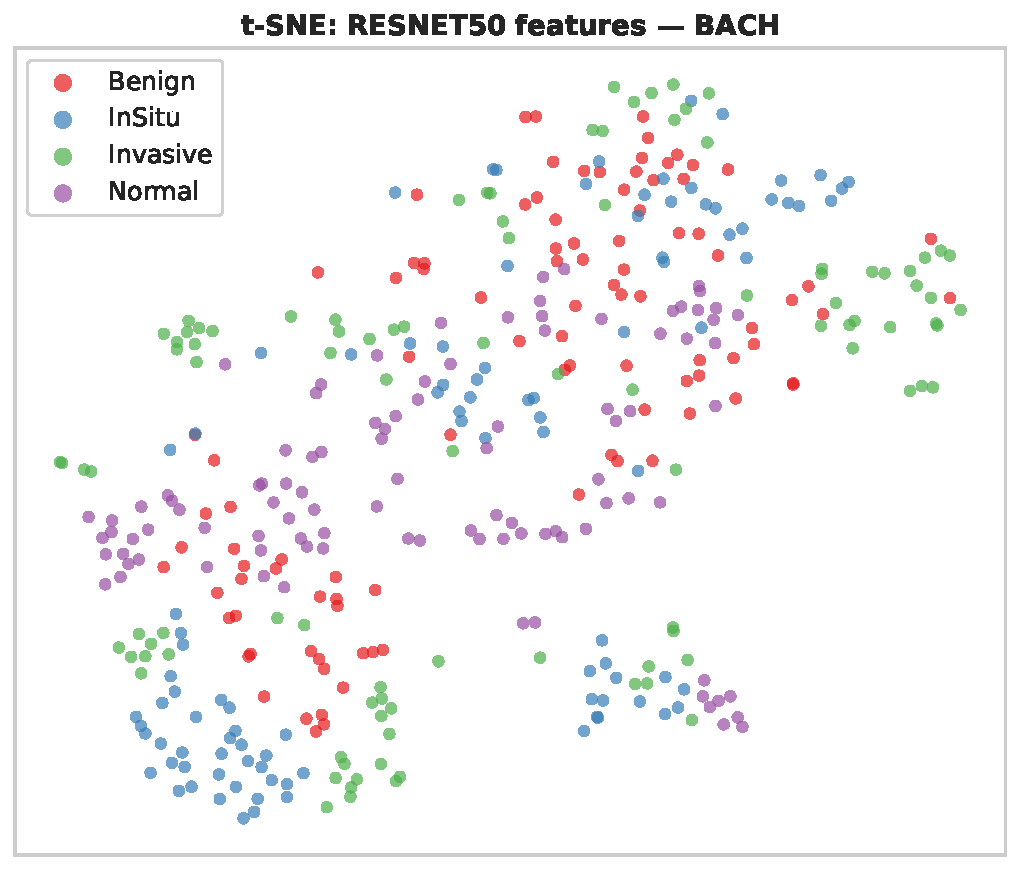
\includegraphics[width=\linewidth]{tsne_resnet50_bach.pdf}
  \caption{t-SNE projection of bag-level mean-pooled ResNet-50 features on BACH.}
  \label{fig:tsne}
\end{figure}

CLAM-SB underperforms both AB-MIL and TransMIL with ResNet-50 despite instance-level supervision---with only 320 training bags per fold, the clustering signal introduces noise rather than sharpens attention, unlike the larger-scale settings where CLAM's advantage is established \cite{lu2021data}.

\subsection{Cross-Domain Results}

Table~\ref{tab:cross_domain} shows cross-domain results for AB-MIL under each TTA strategy. On S1 (BACH$\rightarrow$BACH held-out), all methods reach 1.0000 accuracy under both backbones---an expected ceiling given strong source convergence and the small validation set ($n=80$).

On S2 (BACH$\rightarrow$BreakHis), the results are unambiguous. With ResNet-50, no-TTA accuracy is 0.4590. The best TTA method (TTT-MIL) reaches 0.4591---a change of one image out of 7,909. With UNI, no-TTA accuracy is 0.3339, and all TTA methods land at exactly the same value. Paired McNemar's tests return $\chi^2 = 0.000$, $p = 1.00$ across every method, backbone, and scenario combination. The null hypothesis cannot be rejected in any case.

\begin{table}[!hbt]
\caption{Cross-Domain Accuracy: AB-MIL Under TTA}
\label{tab:cross_domain}
\centering
\begin{tabular}{llccc}
\toprule
\textbf{Backbone} & \textbf{Method} & \textbf{Acc.} & \textbf{F1} & \textbf{AUROC} \\
\midrule
\multicolumn{5}{l}{\textit{S1: BACH $\rightarrow$ BACH held-out (n=80)}} \\
ResNet-50 & All methods & 1.0000 & 1.0000 & 1.0000 \\
UNI & All methods & 1.0000 & 1.0000 & 1.0000 \\
\midrule
\multicolumn{5}{l}{\textit{S2: BACH $\rightarrow$ BreakHis 200X (n=7,909)}} \\
\multirow{5}{*}{ResNet-50}
 & No TTA        & 0.4590 & 0.4586 & --- \\
 & TENT-MIL      & 0.4588 & 0.4585 & 0.5472 \\
 & TTT-MIL       & \textbf{0.4591} & \textbf{0.4587} & 0.5472 \\
 & CORAL-MIL     & 0.4590 & 0.4586 & 0.5472 \\
 & Hybrid-TTA    & 0.4587 & 0.4584 & 0.5472 \\
\midrule
\multirow{5}{*}{UNI}
 & No TTA        & 0.3339 & 0.2779 & --- \\
 & TENT-MIL      & 0.3339 & 0.2779 & 0.5181 \\
 & TTT-MIL       & 0.3339 & 0.2779 & 0.5181 \\
 & CORAL-MIL     & 0.3339 & 0.2779 & 0.5181 \\
 & Hybrid-TTA    & 0.3339 & 0.2779 & \textbf{0.5182} \\
\bottomrule
\multicolumn{5}{l}{All McNemar tests: $\chi^2 = 0.000$, $p = 1.00$.} \\
\multicolumn{5}{l}{``---'': AUROC undefined (single-class predictions at baseline step).} \\
\end{tabular}
\end{table}

%\begin{figure}[!hbt]
  %\centering
  %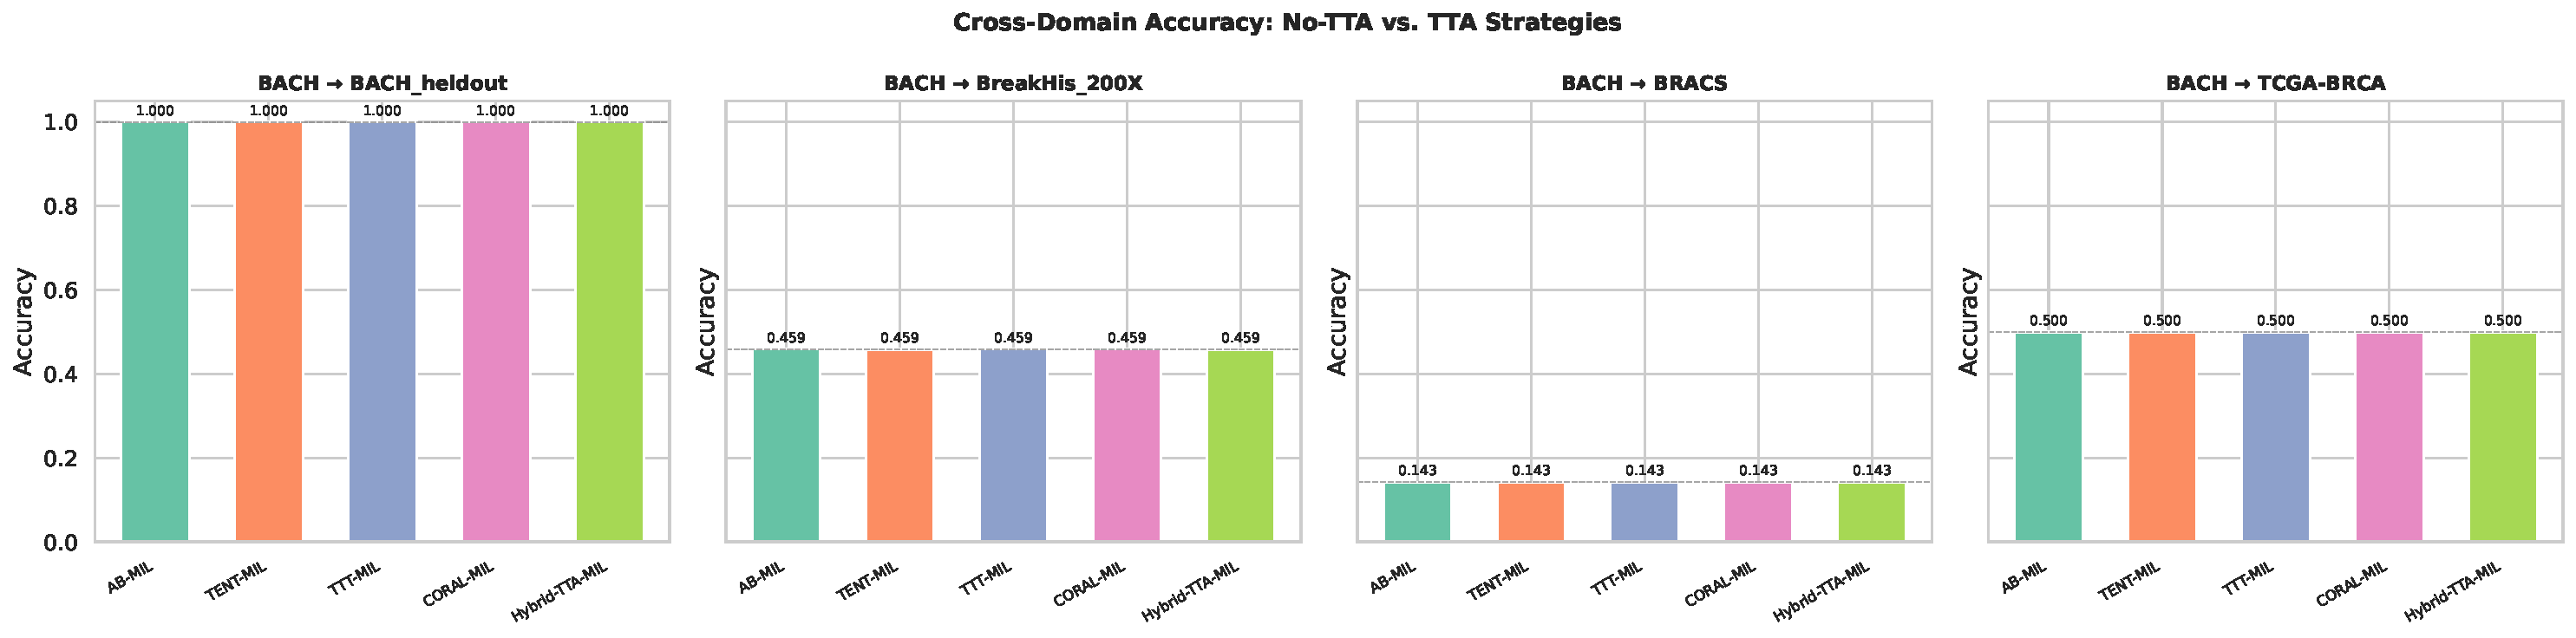
\includegraphics[width=\linewidth]{main_results.pdf}
 % \caption{Cross-domain accuracy of TTA-MIL variants (BACH as source). The dashed line marks the no-adaptation baseline. All four TTA strategies are indistinguishable from the baseline on BreakHis 200X, with differences $\leq$0.0004 accuracy points.}
  %\label{fig:main_results}
%\end{figure}

\subsection{Ablation Study}

Table~\ref{tab:ablation} reports ablation results on the 600-sample stratified BreakHis subset. For ResNet-50, all label-free methods (A1--A5) collapse to 0.0933---complete single-class collapse from a degenerate random head. For UNI, label-free methods reach 0.1883--0.1917, above this floor but far below chance: UNI's structured features create mild incidental variation under random projection, but not enough for any TTA method to exploit. Variation across A1--A5 within each backbone is smaller than sampling variance.

A6 (supervised fine-tuning with 30\% labeled target data) breaks sharply from this pattern: 0.8533 accuracy with ResNet-50 and 0.9250 with UNI. The gap between label-free TTA and supervised fine-tuning is 0.74 accuracy points. TTA closes less than 0.5\% of that gap.

\begin{table}[!hbt]
\caption{Ablation Study on BreakHis (600-sample stratified subset)}
\label{tab:ablation}
\centering
\begin{tabular}{lp{0.12\linewidth}cc}
\toprule
\textbf{Condition} & \textbf{Steps} & \textbf{Acc. (R50)} & \textbf{Acc. (UNI)} \\
\midrule
A1: No TTA           & 0    & 0.0933 & 0.1883 \\
A2: TENT             & 1    & 0.0933 & 0.1900 \\
A3: TENT             & 10   & 0.0933 & 0.1917 \\
A4: TTT              & 5    & 0.0933 & 0.1900 \\
A5: CORAL            & 5    & 0.0933 & 0.1900 \\
\midrule
A6: Fine-tune$^\dagger$ & 5 ep & 0.8533 & \textbf{0.9250} \\
\bottomrule
\multicolumn{4}{l}{$^\dagger$Uses 30\% labeled target samples; not a fair comparison.} \\
\end{tabular}
\end{table}

\begin{figure}[!hbt]
  \centering
  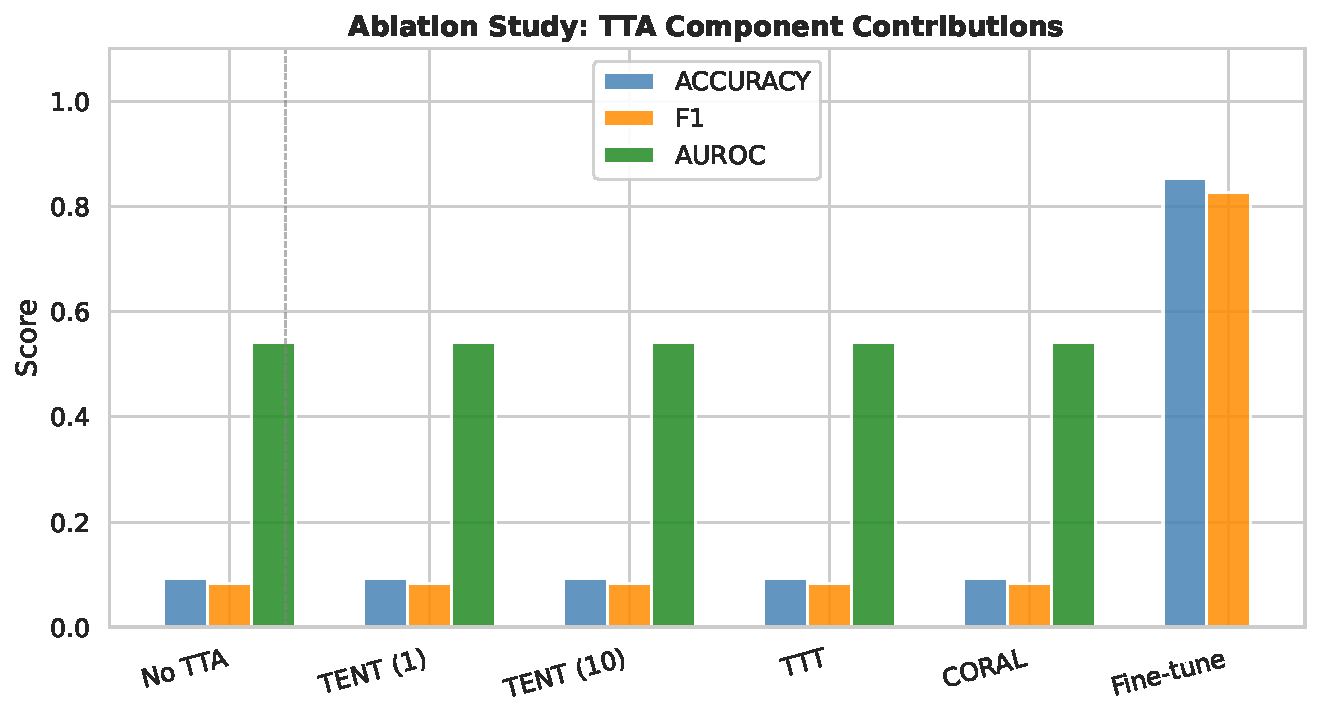
\includegraphics[width=\linewidth]{ablation_results.pdf}
  \caption{Ablation study on BreakHis (600-sample stratified subset).}
  \label{fig:ablation}
\end{figure}

\section{Diagnostic Analysis}
\label{sec:discussion}

\subsection{Root Cause: Random Head Initialization}

BACH trains a 4-class linear head; BreakHis requires a 2-class head. At transfer time, the source head is discarded and a new 2-class layer is randomly initialized. TTA then updates only LayerNorm affine parameters ($\gamma$, $\beta$)---these control intermediate normalization but cannot change the output mapping when it is random. Backpropagated gradients are dominated by noise from the random head, not meaningful class boundaries.

This explains the ResNet-50 single-class collapse (0.0933): entropy minimization produces no useful gradient. UNI features reach 0.19 due to incidental class separation under random projection, but TTA cannot exploit it.

The A6 result confirms the features are adequate: supervised fine-tuning with 30\% labeled target data reaches 0.9250 with UNI. Only the output mapping needed proper fitting.

\begin{figure}[!hbt]
  \centering
  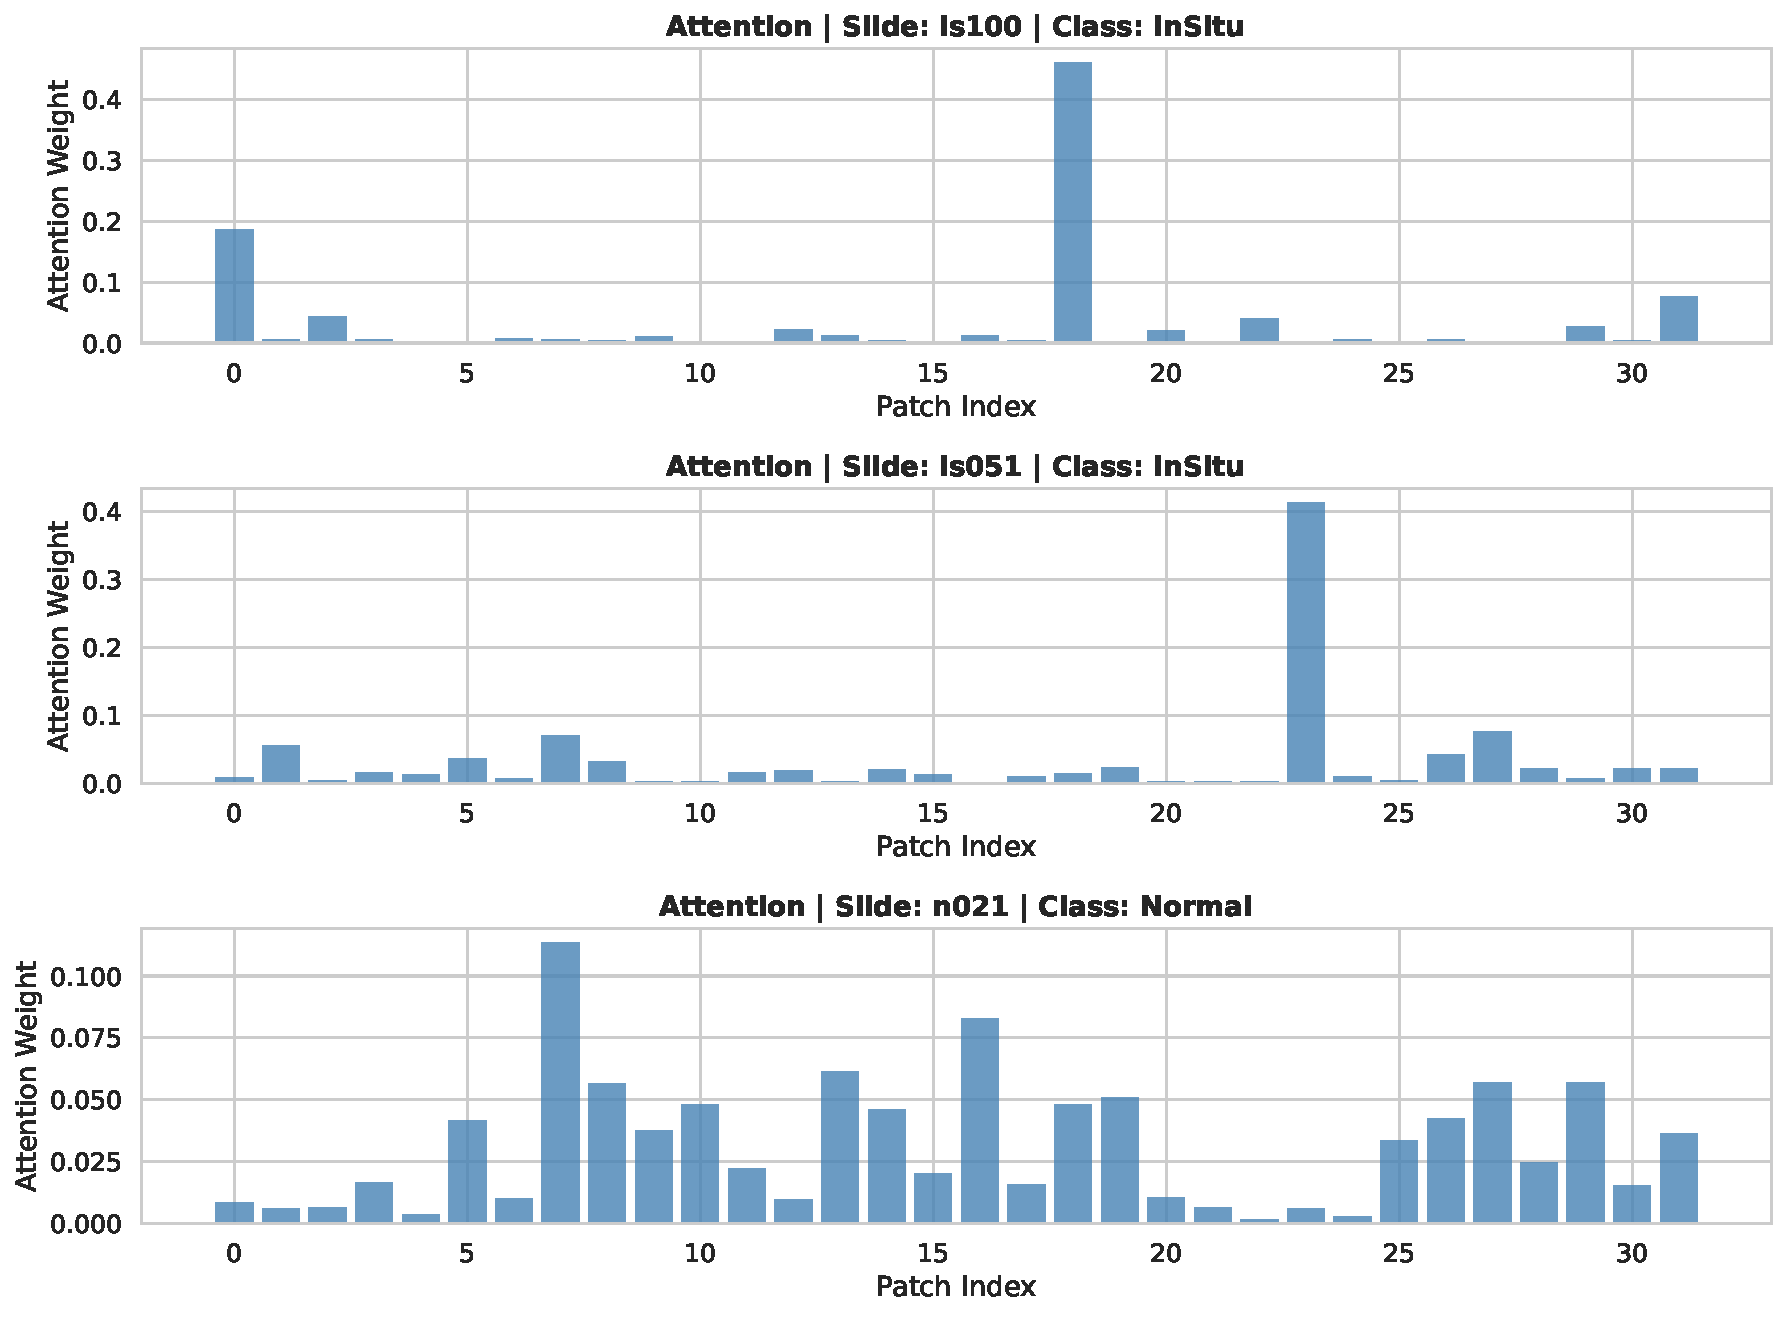
\includegraphics[width=\linewidth]{attention_maps.pdf}
  \caption{Attention weight distributions over patches for three representative BACH slides (AB-MIL, UNI features).}
  \label{fig:attention}
\end{figure}

\subsection{The UNI Paradox}

UNI features produce lower cross-domain baseline accuracy (0.3339) than ResNet-50 features (0.4590) despite dramatically outperforming ResNet-50 on the source domain (0.9700 vs.\ 0.8475). This inverse relationship is worth examining.

UNI's 1024-dimensional features encode fine-grained H\&E-specific texture that maps cleanly onto the 4-class BACH taxonomy. A random 2-class linear layer then cuts through this more complex manifold with a random hyperplane, degrading performance more severely than for ResNet-50's more diffuse 2048-dimensional features. Stronger domain-specific encoders suffer more from head replacement than weaker general-purpose ones---a practical warning for cross-task deployment.

\subsection{Preconditions for TTA in MIL Settings}

Based on this analysis, three conditions must hold before TTA can improve cross-domain MIL performance:

\begin{enumerate}
    \item \textbf{Label-space compatibility:} Source and target must share the same label space, or the source head must be directly transferable (e.g., a superclass-to-subclass or subclass-to-superclass mapping where the head can be pruned rather than replaced). A randomly re-initialized head removes all gradient signal from the TTA objective.

    \item \textbf{Non-trivial source initialization:} The source model must produce non-random predictions on target samples before adaptation begins. If initial AUROC is near 0.5, entropy minimization lacks a useful gradient direction.

    \item \textbf{Matching adaptation scope and gap type:} If the domain gap is in feature distribution (addressed by CORAL) or normalization statistics (addressed by TENT), LayerNorm-only updates can help. If the gap is in the output mapping, adaptation must include the head.
\end{enumerate}

All three conditions are unsatisfied here. Condition 1 is the binding constraint: fixing the label-space mismatch would enable Conditions 2 and 3, as UNI features should produce non-trivial predictions with a valid source head, and the BACH$\rightarrow$BreakHis feature shift is addressable by CORAL in principle.

\subsection{What Would Work}

Two direct fixes follow from this analysis. First, train with a compatible label space: collapse BACH to binary before training (grouping Normal and Benign as one class, InSitu and Invasive as the other), then transfer directly to BreakHis's benign/malignant taxonomy. This mapping is anatomically meaningful---non-invasive lesions vs.\ invasive/pre-invasive ones---and eliminates the head replacement problem entirely, allowing the trained 2-class head to be transferred as-is. Second, extend TTA scope: update the full aggregator including the classification head, using entropy minimization with sharpening \cite{niu2023towards} or pseudo-label filtering to avoid collapsing to a trivial prediction. The combination of both---label-consistent training plus head-aware TTA---is the most defensible direction for future work.

\section{Conclusion and Future Work}
\label{sec:conclusion}

Test-time adaptation fails to close the cross-domain gap for MIL-based breast histopathology classification in the BACH
→
→BreakHis setting. The cause is clear: standard TTA updates only normalization parameters and cannot recover a randomly re-initialized classification head when source and target label spaces differ. Source-domain performance is strong—UNI-based AB-MIL reaches 0.9700 accuracy and 0.9973 AUROC on BACH—and a supervised upper bound of 0.9250 accuracy on BreakHis (30% labeled data) confirms that features are not the obstacle. Label-free TTA yields only 0.19 accuracy, defining the gap that future label-free methods must address. The three-precondition checklist (Section~\ref{sec:discussion}) provides practical criteria to predict TTA success without full experiments.

Limitations: the label-space mismatch reflects real-world deployment, BRACS and TCGA-BRCA were unavailable in compatible format, and only two backbones were evaluated. Future work should pursue head-aware adaptation that updates the classification head jointly with normalization parameters (e.g., entropy sharpening, pseudo-label filtering), explore parameter-efficient test-time techniques (LoRA, prompt tuning, adapter tuning), and evaluate continual TTA methods (CoTTA, SAR) under label-space-compatible conditions. A direct test of the checklist would be to train BACH as a binary task before transferring to BreakHis.

\bibliographystyle{IEEEtran}
\bibliography{references}

\end{document}